\chapter{Models}
The first deep learning-based object detection models emerged after a
breakthrough in ImageNet Large Scale Visual Recognition Challenge (ILSVRC)
\cite{ILSVRC15} in 2012 when Alex Krizhevsky et al. proposed a deep
and wide CNN classification model \cite{alexnet}. The so-called AlexNet
outperformed traditional state-of-the-art models.  This architecture was
later exploited as a feature extractor for the CNN-based object detection
model R-CNN \cite{rcnn}, which also surpassed the previous best results on
PASCAL Visual Object Classes (PASCAL VOC) dataset 2012 \cite{voc}. Since then,
many CNN-based object detection models have been introduced \cite{odreview}.

Generally, they can be categorized into two types: \bld{one-stage detectors}
and \bld{two-stage detectors}. The latter approach consists of a region
proposal step, followed by classification and bounding box regression. This
means that the model initially generates interesting regions, which are then
analyzed one-by-one. In contrast, one-stage detectors are based on a global
regression and classification, requiring a single pass through the network,
and thus they are usually faster but less accurate. A common property of
both approaches is that we can easily substitute the models' feature extractor.

For our comparison, we have chosen three state-of-the-art models: \bld{Faster
    R-CNN} \cite{fasterrcnn}, \bld{Cascade R-CNN} \cite{cascadercnn}, and
\bld{RetinaNet} \cite{retinanet}. The first one was proposed in 2015, and
it is a well-known example of two-stage detectors. The model is considered
to be well-established as it has a reasonable accuracy/speed trade-off
and is easy to modify. In our work, Faster R-CNN serves as a baseline for
our comparison. The next one, Cascade R-CNN, is an extension to Faster
R-CNN, which improves the performance by addressing some of Faster R-CNN's
caveats. Finally, RetinaNet is a recent one-stage detector, aiming to match
the two-stage detectors' accuracy while preserving one-stage detectors' speed.

We describe the models in detail in the following sections. However, let us
first describe the general architecture of the detectors. The architecture
of models can be divided into two parts: \bld{backbone} and \bld{detection
    head}. The backbone is responsible for computing feature maps from the input
image. The feature maps are then used for predicting the bounding boxes and
classifications by the detection head.

\section{Backbone}
All our models use \bld{ResNet} \cite{resnet} for feature extraction. It
can be further extended with \bld{Feature Pyramid Network (FPN)} \cite{fpn}
that helps with detecting the objects at different scales. We describe each
of these components in the following sections.

\subsection{ResNet}
Deeper neural network architectures are harder to train because of the
disappearing gradient. As the gradient is backpropagated through the network,
the repeated multiplication by values between 0 and 1 makes the gradient
very small, and eventually, it vanishes. Thus the earlier layers (closer
to the input) are not trained properly. This is called the \bld{vanishing
    gradient problem}.

ResNet is a CNN-based image recognition model proposed in 2015 \cite{resnet}
to solve the difficulties of training deeper architectures by introducing
\bld{skip connections} between the layers allowing to train up to 1001-layer
deep architectures. For comparison, the previous state-of-the-art model
VGG \cite{vgg} consists of up to 19 sequentially stacked layers (see
\myref{Figure}{fig:vgg_resnet}).

\begin{figure}[h]
    \centering
    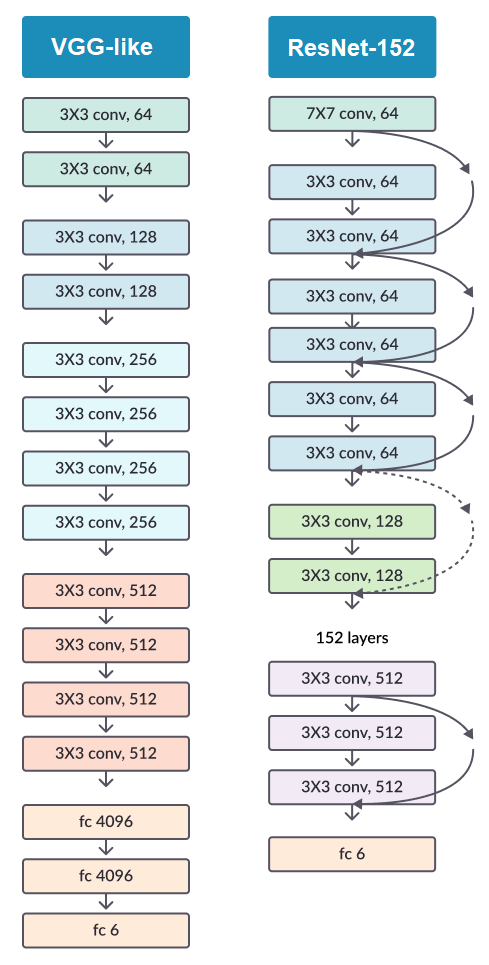
\includegraphics[width=0.5\linewidth]{Sources/Figures/vgg_resnet.png}
    \caption{A visual comparison of a VGG-like network and ResNet. Adapted from
        \cite{resnet}.}
    \label{fig:vgg_resnet}
\end{figure}

Skip connections are realized by performing identity mapping. Its
outputs are then simply added to the outputs of the stacked layers (see
\myref{Figure}{fig:residual_block}). This helps with propagating the gradient
deeper in the network.

\begin{figure}[h]
    \centering
    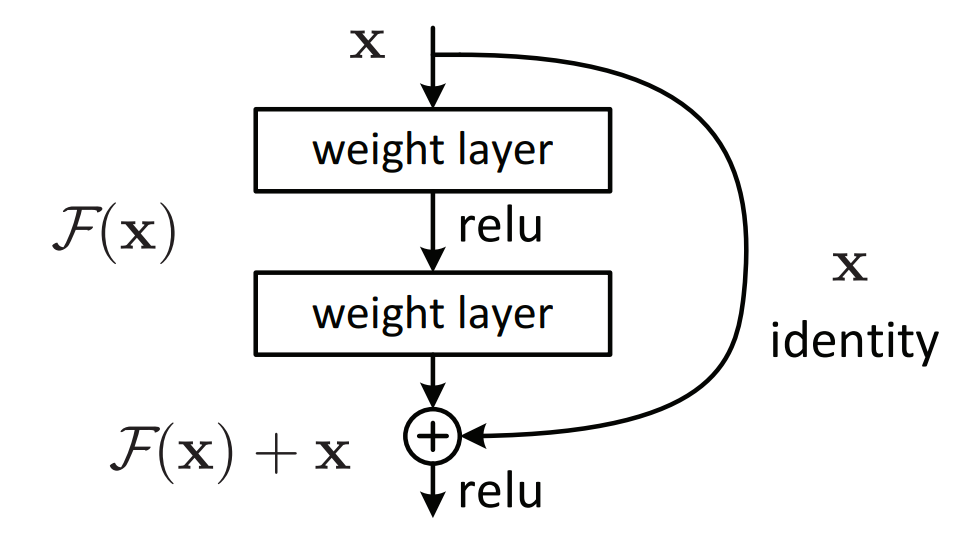
\includegraphics[width=0.4\linewidth]{Sources/Figures/residual_block.png}
    \caption{Visualization of a skip connection \cite{resnet}.}
    \label{fig:residual_block}
\end{figure}

\subsection{Feature Pyramid Network}
One of the challenges of object detectors is to detect objects at different
scales. To approach this, we can simply process the same image at different
scales. However, this naive method is very inefficient and requires a lot of
computation time and memory. A more efficient way would be to take the computed
feature maps that are already of different scales and use them for the
prediction. But the feature maps closer to the input are composed of low-level
features (e.g., edges), which are not very valuable for accurate predictions.
We can visualize these approaches as a \bld{pyramid} of images or features
(see \myref{Figure}{fig:pyramids}).

\begin{figure}[h]
    \centering
    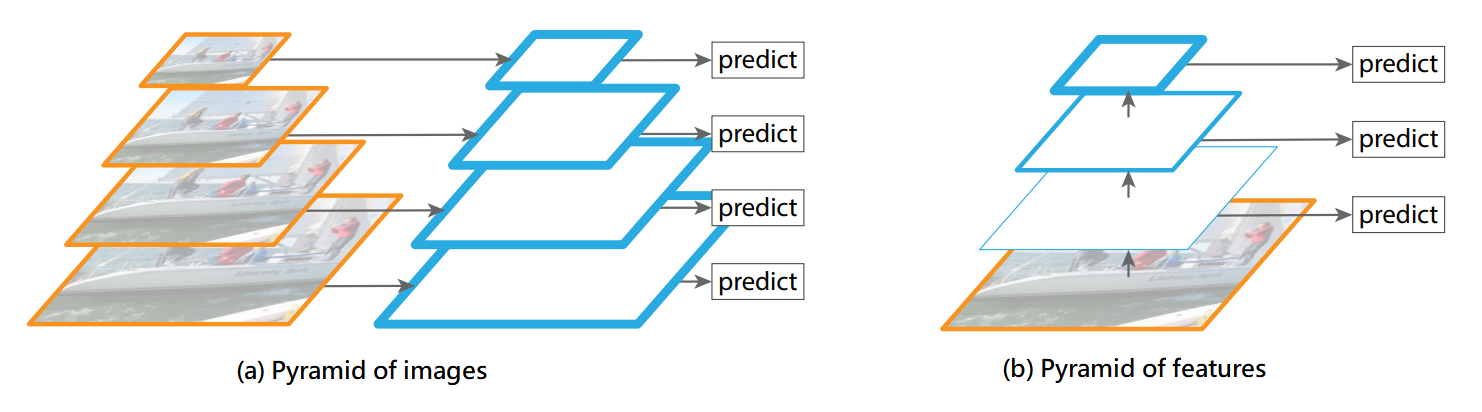
\includegraphics[width=\linewidth]{Sources/Figures/pyramids.png}
    \caption{(a) Features are computed independently for each scale; (b)
        exploits the computed feature maps of feature extractor. Adapted from
        \cite{fpn}.}
    \label{fig:pyramids}
\end{figure}

In 2017 Lin et al. proposed Feature Pyramid Network \cite{fpn}. The
network enhances the feature maps from lower pyramid levels with
high-level features. To achieve this, the construction of the feature
pyramid involves a \bld{bottom-up pathway} and a \bld{top-down pathway}
(see \myref{Figure}{fig:fpn}). The bottom-up pathway is a conventional CNN
feature extractor, which gradually produces smaller and smaller feature maps,
but with high-level features (we say that they are semantically richer). The
top-down pathway upsamples the semantically richer features to match the
higher resolution of the bottom-up pathway feature maps. These different
feature maps are then added together via \bld{lateral connections} between
them. Those connections also help to make training easier, similarly as
in ResNet.  Finally, these semantically enriched multi-scale feature maps
can be used by the detection head of an object detection model.

\begin{figure}[h]
    \centering
    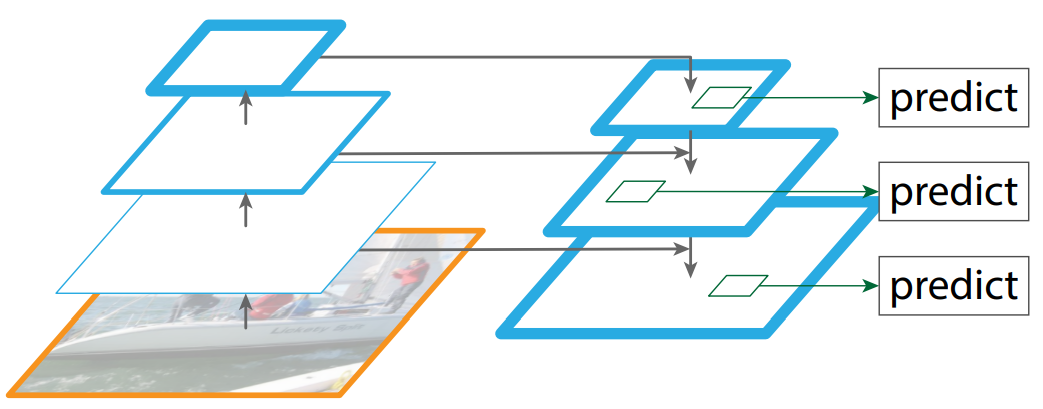
\includegraphics[width=0.6\linewidth]{Sources/Figures/fpn.png}
    \caption{FPN with bottom-up pathway (left), top-down pathway (right) and
        lateral connections (horizontal arrows) \cite{fpn}.}
    \label{fig:fpn}
\end{figure}

\section{Faster R-CNN}
The first model we describe is Faster R-CNN proposed in 2015 by the same
co-authors of ResNet \cite{fasterrcnn}. As we mentioned at the beginning
of the chapter, Faster R-CNN is a two-stage detector. Firstly, it generates
candidate \bld{regions of interest} (RoIs or proposals). This step is known
as a region proposal. The regions are then processed in the detection head
that outputs the predicted class and the bounding box's coordinates. For a
high-level description, we visualize the model with a network flow graph as
in \myref{Figure}{fig:fasterrcnn}.

\begin{figure}[h]
    \centering
    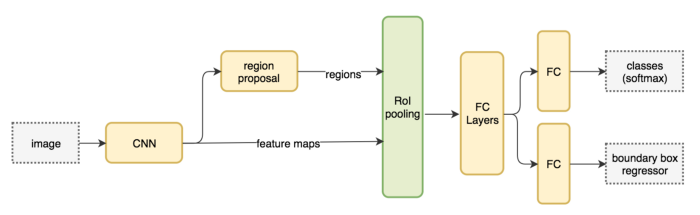
\includegraphics[width=\linewidth]{Sources/Figures/fasterrcnn.png}
    \caption{High-level Faster R-CNN flow. FC stands for fully-connected
        \cite{huifasterrcnn}.}
    \label{fig:fasterrcnn}
\end{figure}

As we can see, Faster R-CNN firstly computes the feature maps, which are
then used by two separate subnetworks. The region proposal is carried out
by a \bld{Region Proposal Network (RPN)}. The corresponding features of
the proposed RoIs are retrieved from the initial feature maps by a method
called \bld{RoI pooling}. The proposals' feature maps are then fed to the
fully-connected network responsible for the final class and bounding box
prediction. We describe each component in detail below.

\subsection{Region Proposal Network}\label{rpn}
A significant part of RPN's architecture resembles a standard CNN image
classifier. The network does not predict the raw coordinates, but instead,
it learns to predict \bld{offsets} of reference boxes. We call these reference
boxes \bld{anchors} (or anchor boxes), and we place them on every point in the
feature map (see \myref{Figure}{fig:rpn}). Each point has several anchors of
different sizes and ratios. We predict an "objectness" score for each anchor,
which is the anchor's probability of being an object. At the same time, we
regress the offsets of the anchors. We determine the ground truth bounding
box with by an \bld{IoU threshold}, i.e., if a proposal overlaps any ground
truth bounding box, then it is assigned to it. Since we now have a large set
of proposals that can overlap, we apply \bld{Non-Maximum Suppression (NMS)}
to solve the issue of duplicates. NMS is a greedy method that goes through
the list of proposals sorted by score and removes proposals with an IoU larger
than the predefined threshold with a proposal that has a higher score. Finally,
the network outputs top $n$ proposals ($n = 2000$ in original paper).

\begin{figure}[h]
    \centering
    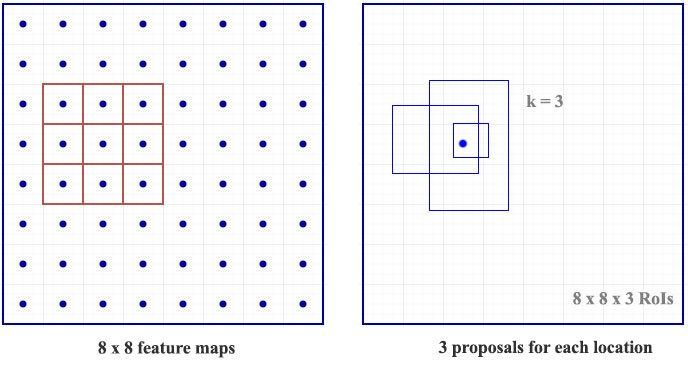
\includegraphics[width=0.625\linewidth]{Sources/Figures/rpn.jpeg}
    \caption{In this illustration, for each point we generate three proposals
        based on the 3 $\times$ 3 features around the point \cite{huifasterrcnn}.}
    \label{fig:rpn}
\end{figure}

\subsection{RoI Pooling}
Once we have proposals of different sizes and ratios, we need to convert
maps to their corresponding features to fixed-size feature maps because the
fully-connected network has a fixed-length input by definition. The conversion
is done by \bld{RoI pooling layer} that takes the input proposals and outputs
fixed-size feature maps.  For every input proposal, crop the corresponding
section in the input feature map. If we need a $w \times h$ output feature
map, we equally divide the section into $w \times h$ blocks. We then apply
max-pooling for these blocks, creating a new $w \times h$ feature map. For
illustration, see \myref{Figure}{fig:roipooling}.
\begin{figure}[h]
    \centering
    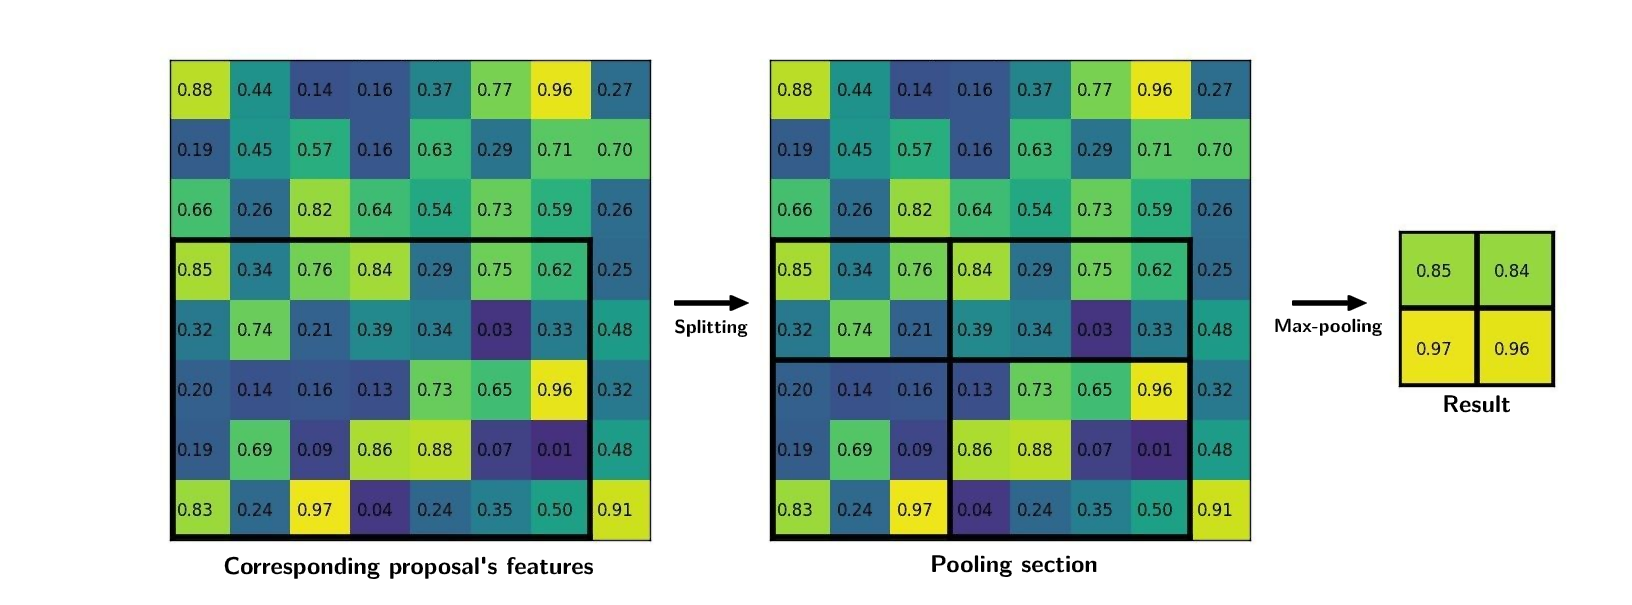
\includegraphics[width=1.05\linewidth]{Sources/Figures/roi.png}
    \caption{Illustration of RoI pooling outputting a $2\times 2$ feature map.
        \cite{roipooling}}
    \label{fig:roipooling}
\end{figure}

\subsection{Fully-connected Layers}
Each output of the RoI pooling layer is flattened (i.e., if we have a
tensor of shape $w \times h\times channels$, we reshape it to a $w \cdot
    h \cdot channels$-dimensional vector) and passed into fully-connected
layers. Similarly, as in RPN, these layers are responsible for adjusting the
bounding box coordinates and category prediction (in RPN we only predicted
if the proposal contains an object or not). The ground truth bounding boxes
are determined similarly as in RPN. The IoU threshold value is usually set
to 0.5. The component's architecture is visualized in \myref{Figure}{fig:rcnn}.

\begin{figure}[h]
    \centering
    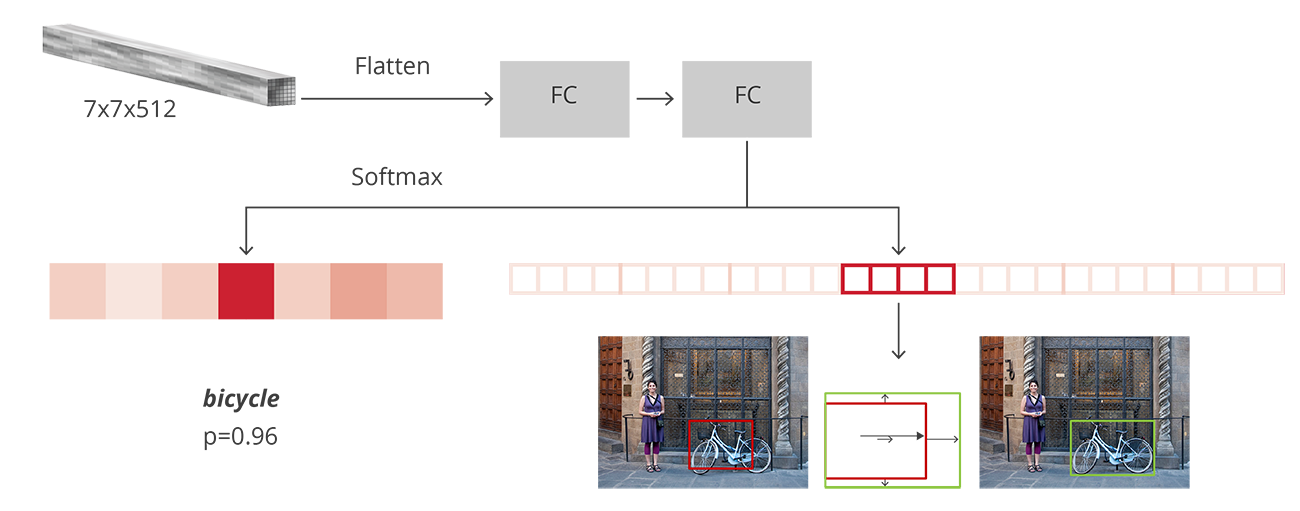
\includegraphics[width=0.95\linewidth]{Sources/Figures/rcnn-architecture.6732b9bd.png}
    \caption{Visualization of classification and regression component \cite{fasterrcnnhead}.}
    \label{fig:rcnn}
\end{figure}

\section{Cascade R-CNN}
As we mentioned in the previous section, Faster R-CNN is trained with a
relatively small IoU threshold value. Such a low threshold value produces many
\bld{noisy detections}. However, setting a higher value would cause the detector
to miss a lot of objects. This problem is addressed by an architecture
proposed in 2017 by Cai et al. \cite{cascadercnn}. They observed that the
output of a detector trained with a certain IoU threshold is a good set
of proposals to train the detector of the next higher IoU threshold. The
architecture extends the Faster R-CNN's detection head by adding a sequence
of detection heads with increasing IoU thresholds. Since the architecture's
detection head resembles a \bld{cascade} (see \myref{Figure}{fig:cascade}),
the authors call it Cascade R-CNN. This enhancement achieved better results
on a COCO dataset \cite{coco} than a simple Faster R-CNN architecture.

\begin{figure}[h]
    \centering
    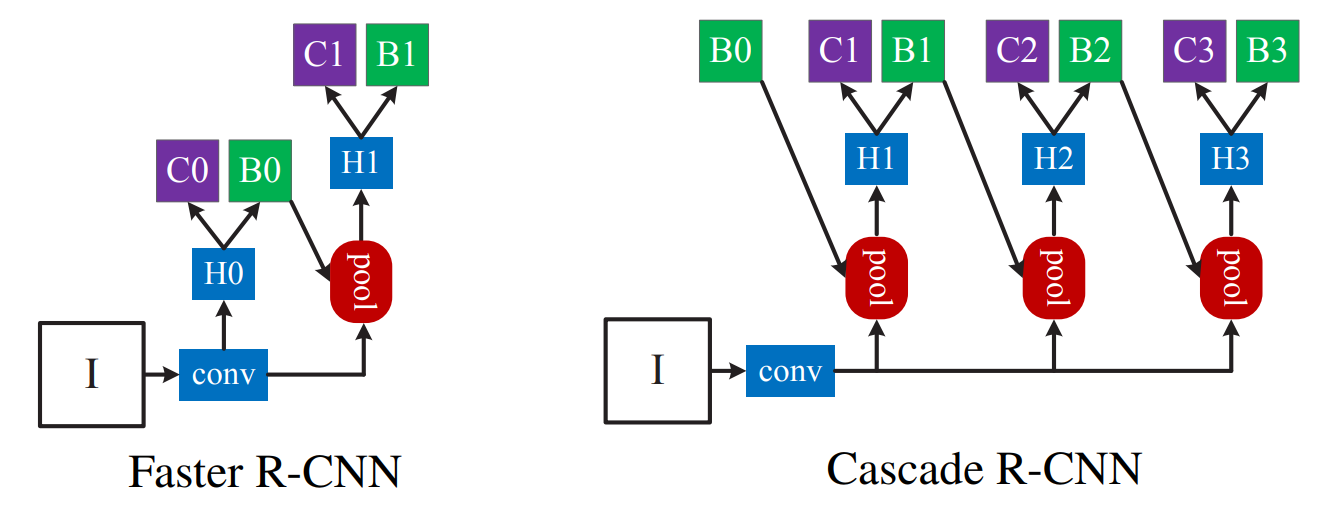
\includegraphics[width=0.85\linewidth]{Sources/Figures/cascade.png}
    \caption{Illustration of different architectures. "I" is input, "H" is
        fully-connected layers, "C" is classification, "B" is proposals, "conv" is
        backbone convolutions, "pool" is RoI pooling \cite{cascadercnn}}
    \label{fig:cascade}
\end{figure}

\section{RetinaNet}
The last model we use is a one-stage detector. One-stage detectors achieve
faster inference speed than two-stage detectors by \bld{skipping the region
    proposal stage}, predicting the bounding boxes and categories directly
in a single pass. One-stage detectors tend to have worse accuracy than
two-stage detectors.  However, recent proposals of new one-stage architectures
achieve similar accuracy while maintaining the faster speed \cite{retinanet,
    yolo3}. This section covers the architecture of a detector called RetinaNet
proposed by Lin et al. in 2018.

Its architecture resembles RPN (recall \myref{Section}{rpn}). However, instead
of predicting the objectness score, it predicts the final class. It also uses
anchor boxes similar to those in RPN. The backbone of RetinaNet is based on
ResNet with FPN extension. Every FPN pyramid level is then connected to two
subnetworks: a class prediction subnetwork and a bounding box regression
subnetwork. These subnetworks are \bld{fully-convolutional}. That means
they do not contain any fully-connected layers, making it possible to feed
in inputs of variable size. See \myref{Figure}{fig:retinanet} for an illustration
of the architecture.

\begin{figure}[h]
    \centering
    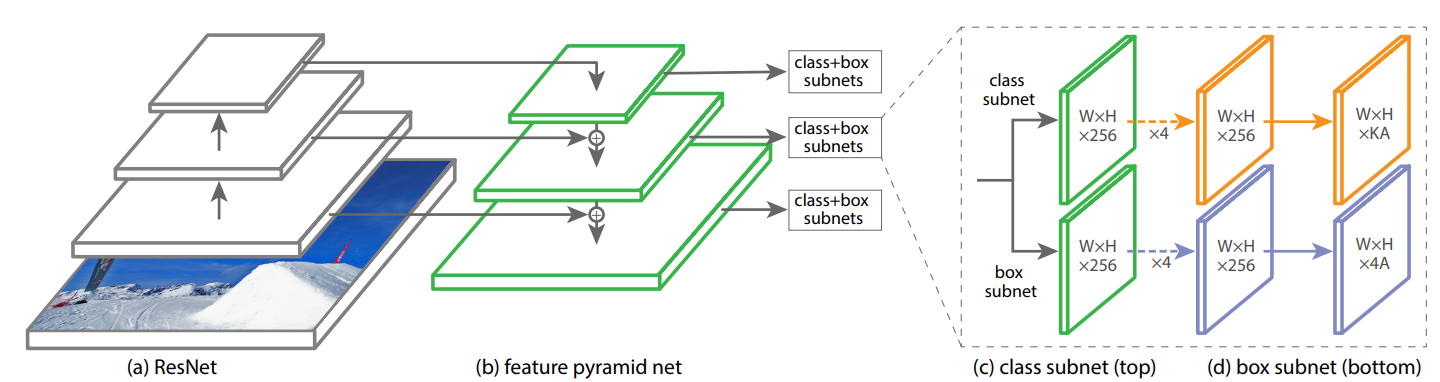
\includegraphics[width=\linewidth]{Sources/Figures/retinanet.png}
    \caption{RetinaNet's architecture. (a) and (b) form the backbone, while (c)
        and (d) are responsible for the class prediction and box regression
        \cite{retinanet}.}
    \label{fig:retinanet}
\end{figure}

RetinaNet was designed to evaluate the effectiveness of a newly proposed
\bld{focal loss} function that improves the training. The authors observed that
previous one-stage detectors \cite{yolo1, yolo2, ssd} suffer from extreme
\bld{foreground-background class imbalance}. This means that the networks
generate a vast number of anchor boxes, while the majority of them do not
contain any object. The authors discovered this issue hurts the training as the
detector rather learns to detect the background instead of being taught to
detect the actual objects. They address this problem by reshaping the standard
cross-entropy loss, so it down-weights the loss assigned to
\bld{well-classified examples}, since most of those examples are just the
background examples.

For simplicity, lets consider a \bld{cross-entropy (CE)} loss for binary
classification:
\[
    \text{CE}(p, y) = \left\{
    \begin{array}{ll}
        -\log(p)   & \text{if } y = 1  \\
        -\log(1-p) & \text{otherwise.} \\
    \end{array}
    \right.
\]
Where $y = \{-1, 1\}$ is representing the \bld{ground-truth class} and
$p \in [0, 1]$ is the model's \bld{estimated probability for the class $y = 1$}.
For convenience, we define $p_t$:
\[
    p_t = \left\{
    \begin{array}{ll}
        p   & \text{if } y = 1  \\
        1-p & \text{otherwise.} \\
    \end{array}
    \right.
\]
We then simplify $\text{CE}(p,y) = \text{CE}(p_t) = -\log(p_t)$. The CE loss is
reshaped by adding a \bld{modulating factor} $(1 - p_t)^\gamma$. The
$\gamma \geq 0$ is a tunable parameter which determines the magnitude of
modulation. Finally, we have:
$$
    \text{FL}(p_t) = (1-p_t)^\gamma \log(p_t).
$$
Lets consider that the well-classified examples have $p_t$ near 1. As we can
see, if $p_t$ is near 1, the modulating factor decreases to 0 and down-weights
the loss (see \myref{Figure}{fig:focalloss} with various values for $\gamma$).

\begin{figure}[h]
    \centering
    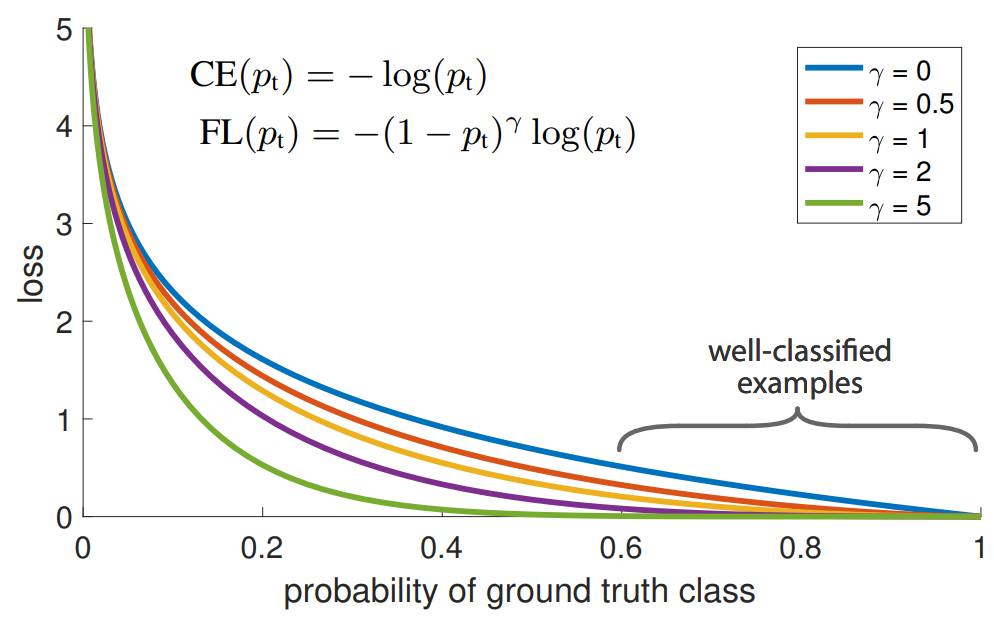
\includegraphics[width=0.7\linewidth]{Sources/Figures/focalloss.png}
    \caption{The focal loss down-weights the loss for well-classified examples.
        If we set $\gamma$ to 0, we get the standard cross-entropy loss
        \cite{retinanet}.}
    \label{fig:focalloss}
\end{figure}

These improvements led to outperforming both one-stage detectors and two-stage
detectors on a COCO dataset \cite{coco}.